\chapter{Exploring the Huff Model\label{ch:huff}}

 We began in Chapter \ref{ch:intro}  what will be a series of studies of business analytics  examples by looking at a quite simple model, Converse's formula for locating a single store in the neighborhood of an incumbent establishment.  The main themes of that chapter---the computational problem solving cycle, the emphasis on post-solution analysis and exploration, the focus on implementation and an analytics dashboard---will be with us throughout the book. They are vey much present in this chapter, where we focus on the Huff model, which can be seen as in the historical line of development ensuing upon Converse's formula.
 
 Besides the Huff model, we introduce in this chapter two new NetLogo models, the distinction between parametric and strategic decision making, greedy hill climbing, and the concept of agent-based modeling. These concepts will be part of our armamentarium going forward.
 

\section{The Huff Model}


%\cite[page 433]{eiselt_marianov_eds_2011}

\subsection{Problem Description}

A number of  establishments that compete for regional customer exist or are contemplated in a particular geographic area.  Given the several locations and attractivenesses of these establishments, we would like to predict the market share each will achieve.  We are interested in deciding  whether to build a number of new establishments as well as where to put any we do decide to build.

This problem falls under the category of \emph{market area analysis,}\index{market area analysis} addressing one of the category's main concerns: the location of prospective retail stores. The Huff model is used extensively for this purpose.

\subsection{Solution Concept}

We use the Huff model as the main basis for our analysis.
The Huff model is expressed mathematically as follows.\index{Huff model}
\begin{equation}
P_{ij} = \frac{\frac{S_j^{\alpha}}{T_{ij}^{\beta}}}{\sum_{j=1}^n\frac{S_j^{\alpha}}{T_{ij}^{\beta}}}\label{exp:huff}\index{Huff model}
\end{equation}
where
\begin{itemize}
\item $P_{ij}$: The probability of a consumer at a given origin $i$ traveling to a particular shopping center $j$.
\item $S_j$: The size of a shopping center $j$ (typically measured in terms of the square footage of selling area devoted to the sale of a particular class of goods). More generally, a measure of attractiveness of the shopping center (with higher values more attractive than lower values).
\item $T_{ij}$: The travel time or cost for customer  $i$ to go to shopping center $j$.
\item $\alpha$: A parameter, to be estimated empirically but often simply set to 1, for scaling the importance of the attractiveness measure for the establishment, $S_j$.
\item $\beta$: A parameter, to be estimated empirically but often simply set to 2 (hence the literature often speaks of the  ``Huff gravity model'' for this class of models), reflecting the effect of travel time and other costs on various kinds of shopping trips.
\item $n$:  The number of establishments or shopping centers under consideration.
\end{itemize}

Further, it is presumed in using this model that there are $m$ customers, that each customer has a known location, and that each of the establishments under consideration has a known location, real or hypothetical.




\subsection{Design}

The model is quite straightforward. Once we represent and record 
\begin{enumerate}
\item the locations of the customers who will potentially visit the establishments,
\item  the locations (real or hypothesized) of the establishments (such as shopping centers) under consideration, and
\item the attractiveness (e.g., size) scores of the establishments under consideration
\end{enumerate}
it is a simple matter to calculate Euclidean distances as the measure of the transportation costs, the $T_{ij}$'s.  Of course, including more realistic measures of transportation costs is a ask that can be arbitrarily onerous. We take this matter up in the discussion section, \S\ref{sec:huff_discussion}.

An organization deciding whether, and if so where, to locate a number of establishments will not be directly interested in the outputs of the Huff model, the $P_{ij}$'s. It simply does not matter what the probability is that a particular individual $i$ will shop at a given store, $j$.  What matters is the overall level of customer traffic. This can be estimated with the Huff model by summing the probabilities for each store over the customers to get the expected traffic for each establishment:
\begin{equation}
 \mbox{expected\_traffic}_j = \sum_{i}^m P_{ij}, \ \ \forall j = 1, 2, \ldots, n
 \end{equation}

\newpage
\subsection{Design \&\ Encoding 1}

Figure \ref{fig:huffnlogo} shows the Interface tab of the  Huff NetLogo model. There are 1000 customers in the region, scattered randomly by the setup procedure and displayed as gray dots. There are four establishments present, represented as black squares. The report in the output widget in the lower left-hand corner of the window tells us that the establishment at location 2, -1 has the highest expected traffic, at 362.92. 

The number and placement of stores in Huff are determined interactively. After initialization with the setup button, the user clicks the add-drop-stores button and clicks to add or delete a store. When finished adding and deleting stores, the user clicks the add-drop-stores button again and proceeds to  evaluate the traffic per store by clicking on the calculate-store-traffic button.  Such is the basic drill with the Huff NetLogo model.\index{Huff.nlogo@{\it Huff.nlogo}} Many  iterations and variations on it are possible for doing interesting analytics.


\begin{figure}[htbp] %  figure placement: here, top, bottom, or page
   \centering
   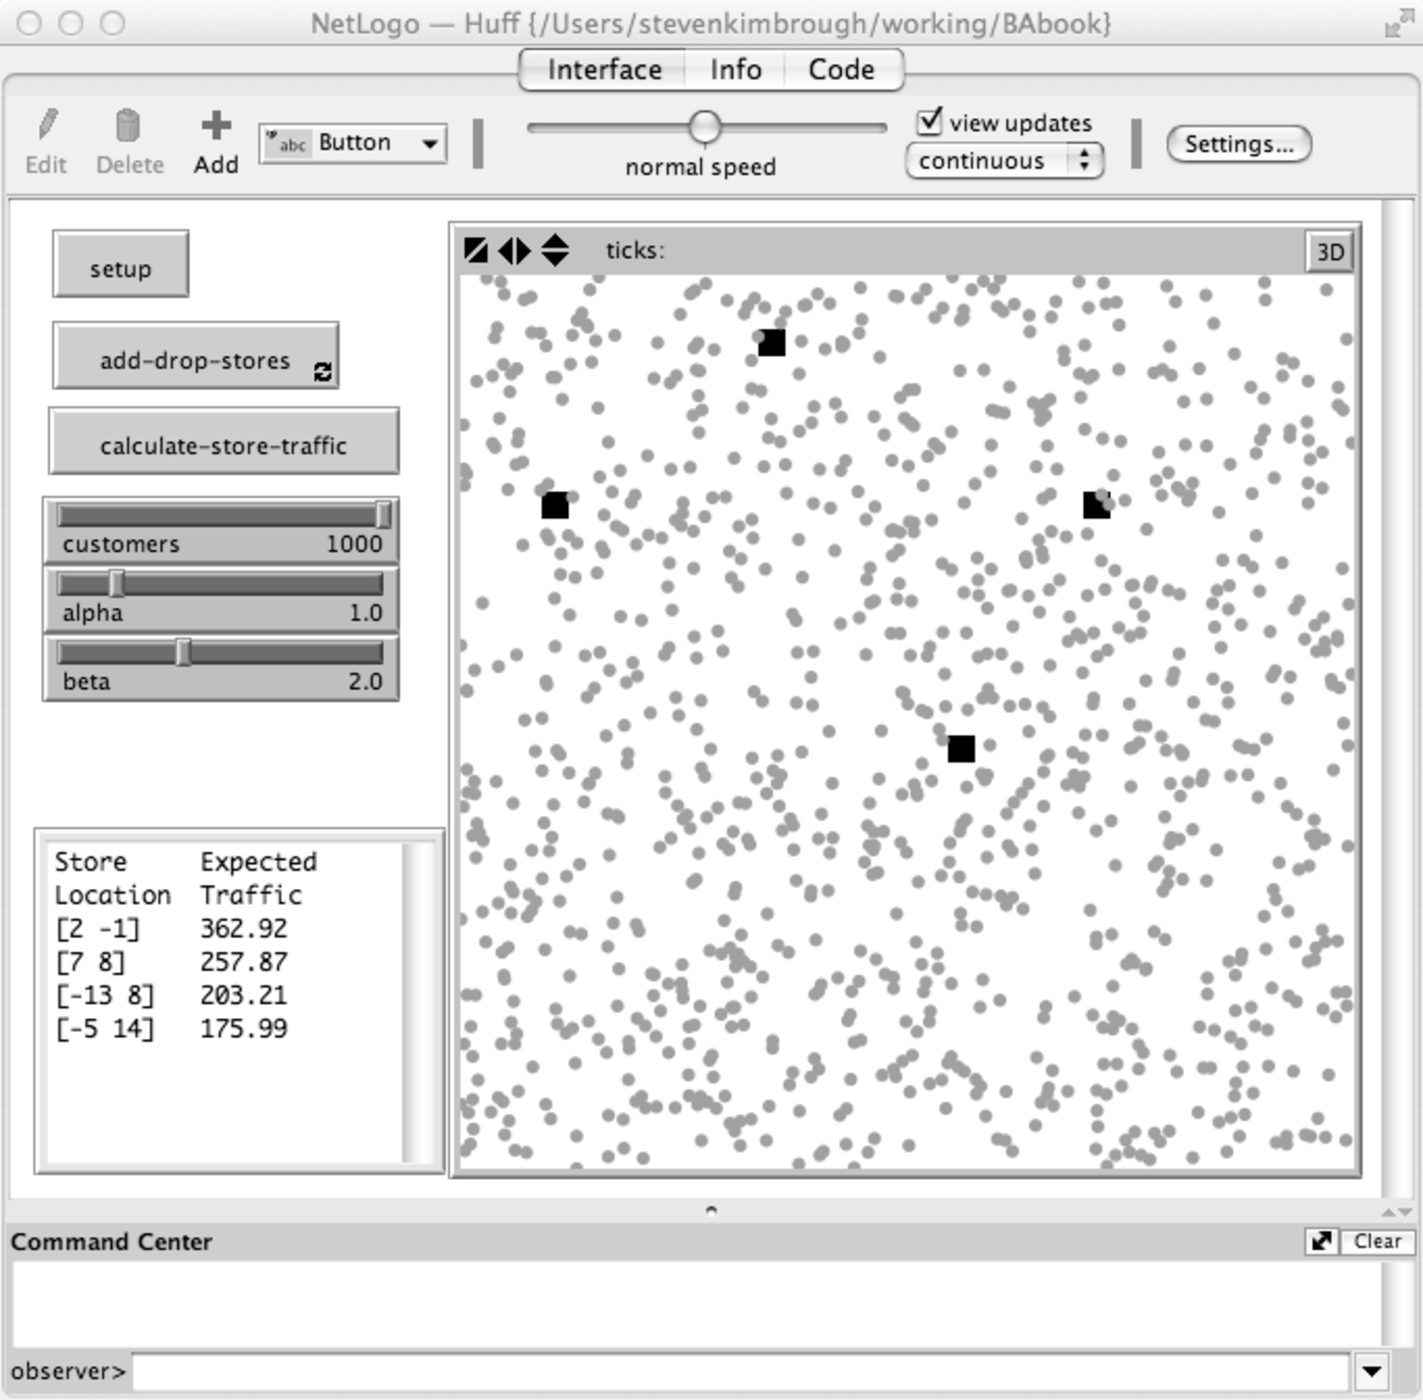
\includegraphics[width=\textwidth]{figures/HuffPatches.pdf}  
   \caption{Huff, a NetLogo implementation of Huff's model.} % using random-seed 22478
   \label{fig:huffnlogo}
\end{figure}
\newpage

Most significantly regarding our design and encoding of the model, the Huff NetLogo model is an ABM, an agent-based model.\index{agent-based model}
Stores, establishments, in Huff NetLogo model are represented by patches\index{NetLogo!patches} whose {\tt store-at?} properties are set (dynamically) to {\tt true}. Customers are represented by turtles. The number of customers is controlled by the customers slider on the Interface tab, shown in Figure \ref{fig:huffnlogo}. The number and placement of stores is, as already described, determined at run time by the user working interactively with the model.  In NetLogo, both patches and turtles are agents. As such, they are potentially rich in capabilities and capacities to act and  to store information. Turtles may move about in the NetLogo world, although they do not do so in the Huff model. Patches are fixed in place, but otherwise are potentially very active and capable agents. NetLogo's world is based upon a two-dimensional grid  of patches, arrayed much as is a checkerboard. Each patch has an address. by default the patch at the center of the world has address 0, 0. Other addresses work like Cartesian co-ordinates with respect to it. For example, in Figure \ref{fig:huffnlogo} reference is made to a store at store location [7 8]. This is the black square (store) that is east of the three other black squares. It is seven patches east of 0, 0 and eight patches north.

\subsection{Employment 1\label{sec:Huff:employment_1}}

The program file for the Huff NetLogo model is {\it Huff.nlogo.}\index{Huff.nlogo@{\it Huff.nlogo}} It is available at the book's web site and at the NetLogo Modeling Commons 
 \url{http://www.modelingcommons.org}.\index{Modeling Commons}
 To run the program you will need to download and install NetLogo on your computer.
The NetLogo home page is \url{https://ccl.northwestern.edu/netlogo/}.\index{Netlogo!home page} There, you can download NetLogo and access a rich corpus of information about NetLogo.

The Huff model, with the customer and store data associated with Figure \ref{fig:huffnlogo}, gives us the expected store traffic for each of the four stores present.  The NetLogo implementation affords exploration of the basic result.  One way to do this is to keep the customers fixed and vary the locations of the stores.  For example, imagine that three stores are presently in operation, those at [7 8] (which is your store), [-13 8], and [-5 14]. The present situation is as shown in Figure \ref{fig:huffnlogo_original_3}. Your store has traffic of about 430, which is expected to drop to about 258 once the new store at [2 -1] comes online. Given this, you might consider relocating your store.  Where would be a more advantageous position for your store? Using the add-drop-stores and calculate-store-traffic buttons in the Huff NetLogo model you can explore for possibilities. For example, if you relocate to  [-9 -3] your expected traffic is 276, an improvement over the 258 you expect if you stay. See Figure \ref{fig:HuffMove1pdf}.

In light of the Huff model, a second way to improve your store's traffic numbers is to increase its size. Starting with the model configuration shown in Figure \ref{fig:HuffMove1pdf}, remove the new store at [-9 -3] by (1) clicking on the add-drop-stores button, (2) clicking on the store's patch (which makes the store disappear, and (3) clicking again on the add-drop-stores button. Now you can re-create your original store as follows:
\begin{enumerate}
\item Type {\tt inspect patch 7 8} after {\tt observer>} in the Command Center then press Enter/Return on your keyboard.

This will produce the window shown in Figure \ref{fig:Huff:inspecting_patch_7_8}.
\item Edit {\tt pcolor} (``patch color'') to change it from 9.9 (white) to 0 (black; you can actually type {\tt black} but NetLogo will change it to 0).
\item Edit {\tt store-at?} to change it from {\tt false} to {\tt true}.
\item Edit {\tt store-size} to change it from 1 to 2.
\item Click on the calculate-store-traffic button.  
\end{enumerate}
Figure \ref{fig:Huff_increased_store_size} shows you what you should get in result.



\begin{figure}[htbp] %  figure placement: here, top, bottom, or page
   \centering
   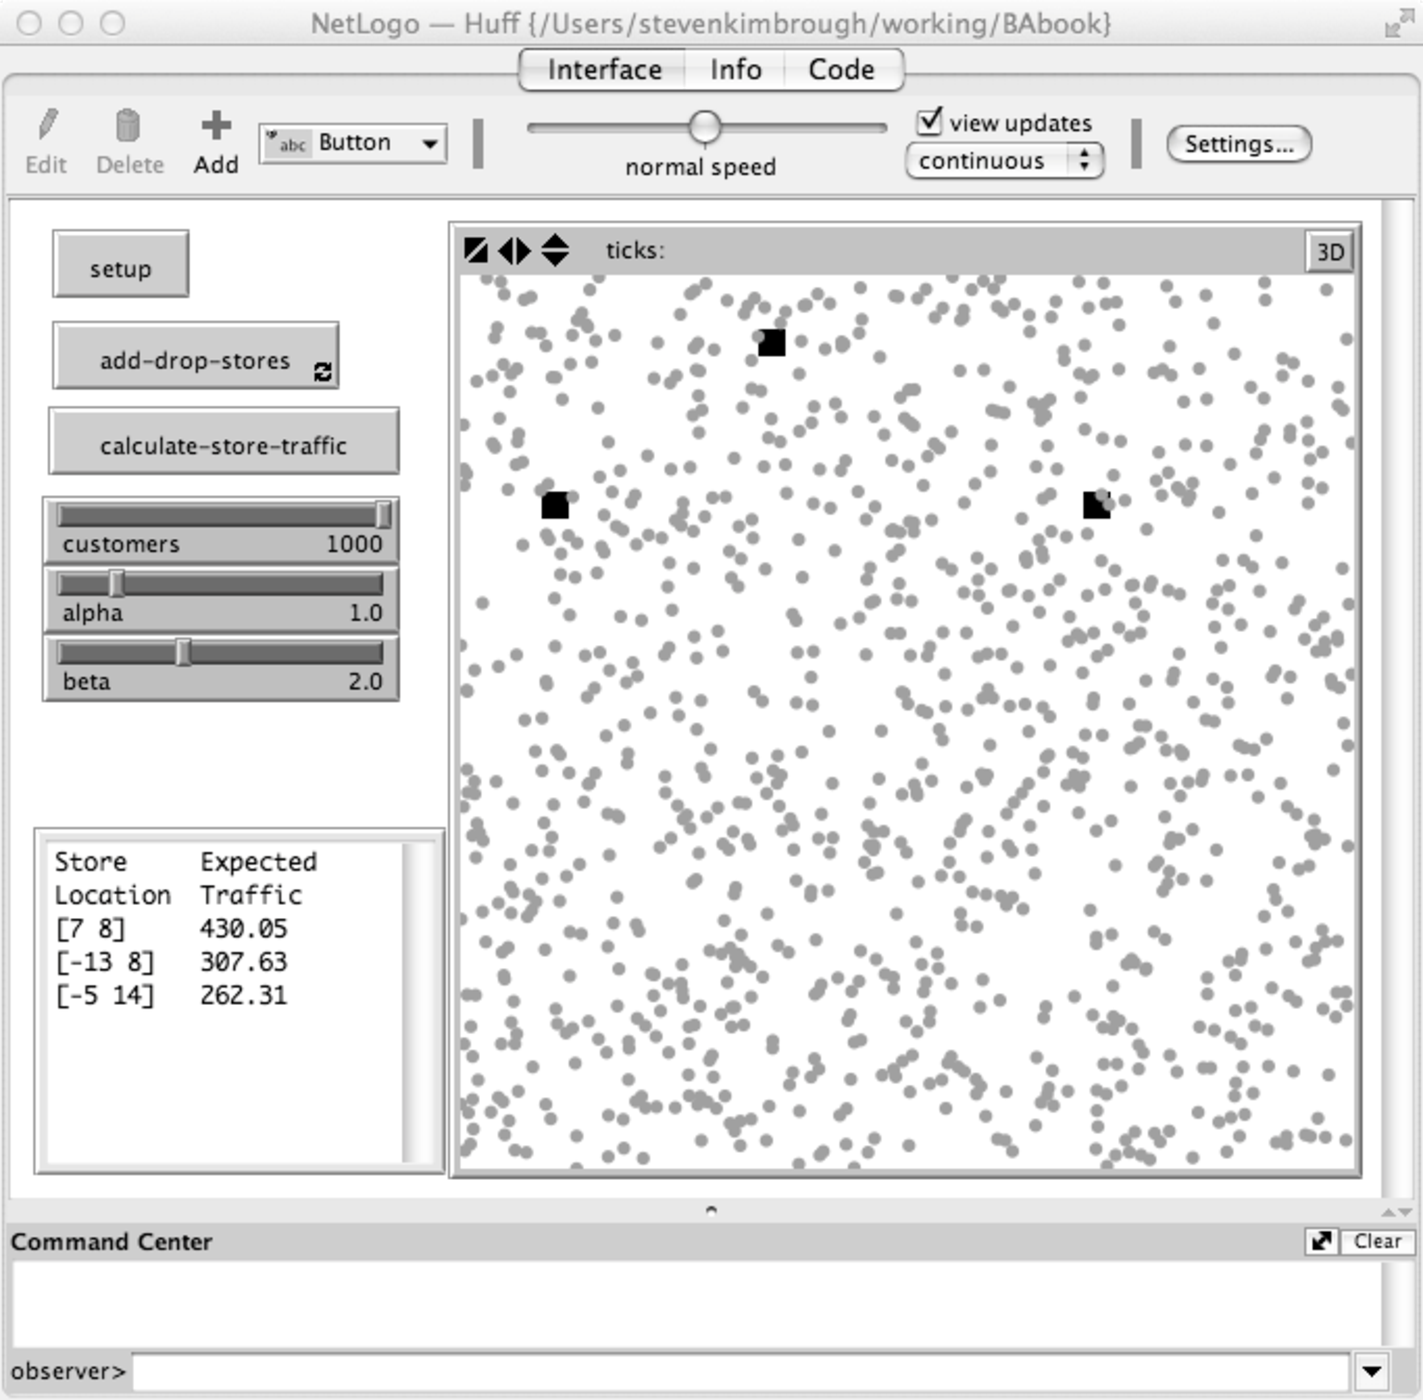
\includegraphics[width=\textwidth]{figures/HuffCase3Start.pdf}  
   \caption{Huff, a NetLogo implementation of Huff's model.} % using random-seed 22478
   \label{fig:huffnlogo_original_3}
\end{figure}



\begin{figure}[htbp] %  figure placement: here, top, bottom, or page
   \centering
   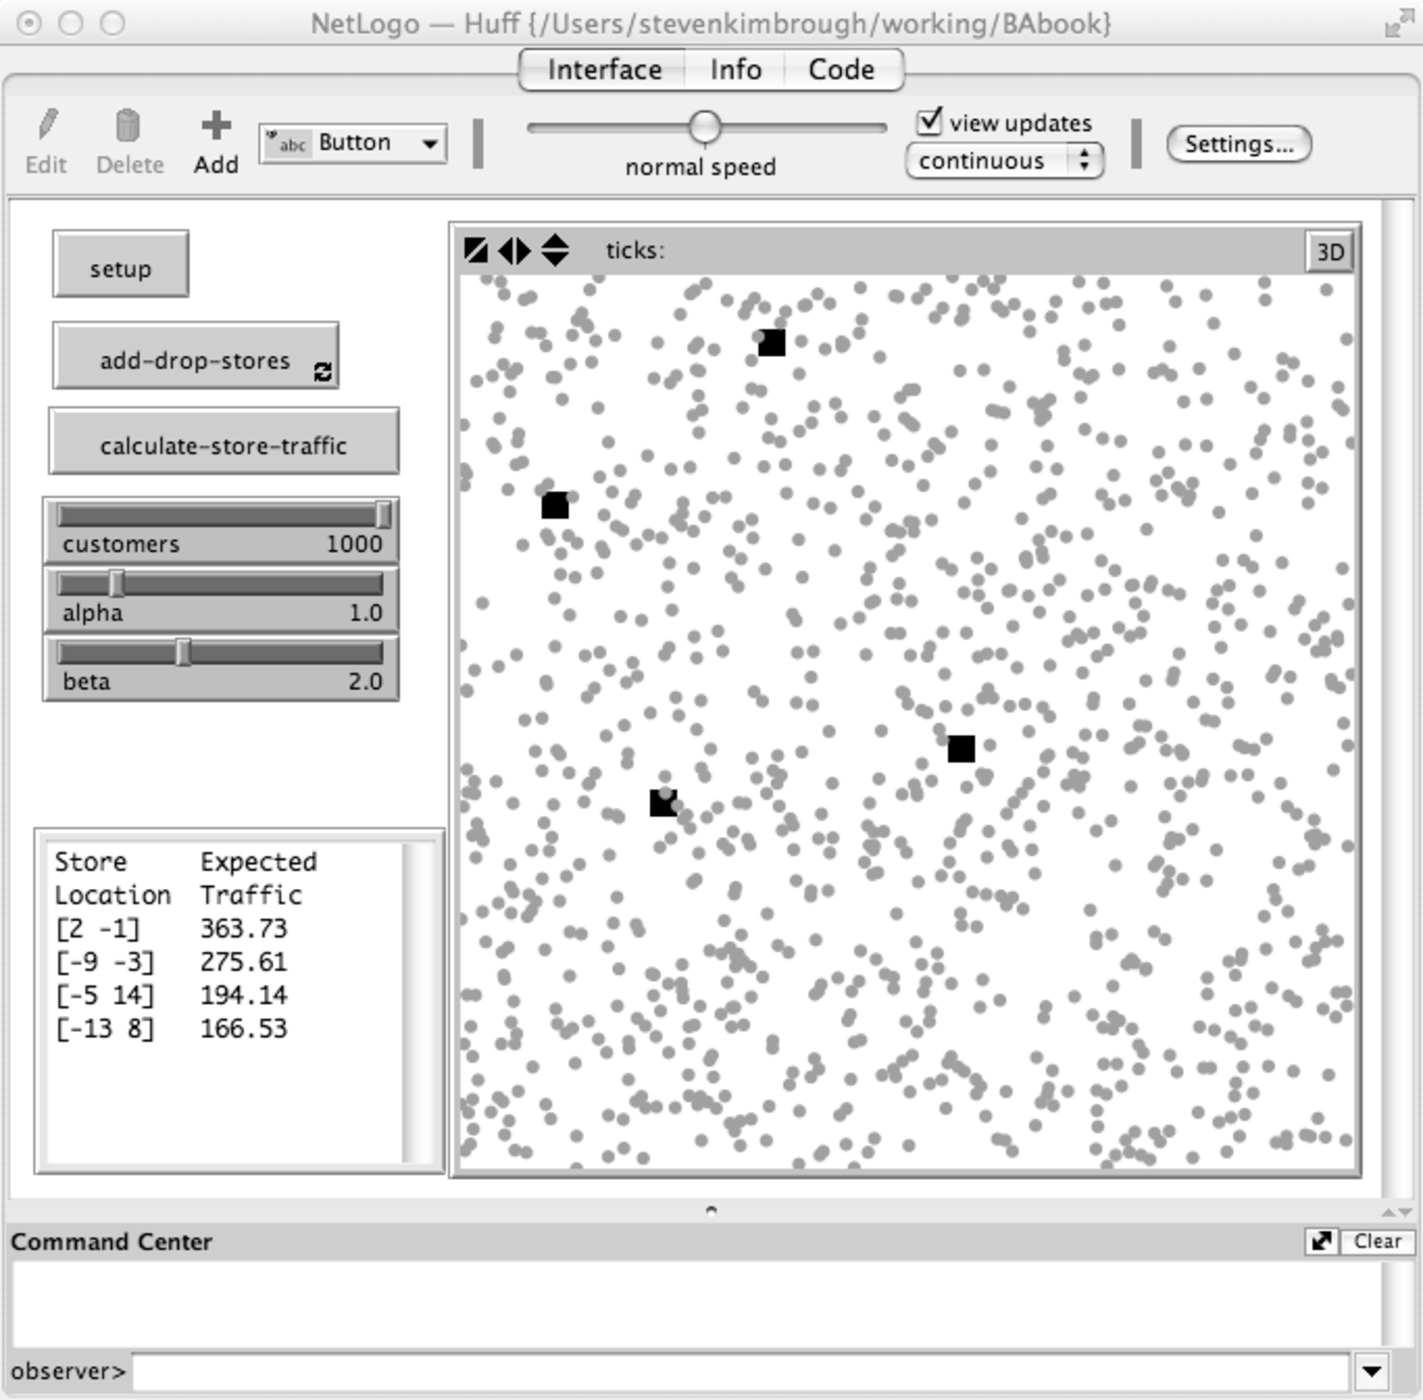
\includegraphics[width=\textwidth]{figures/HuffMove1.pdf}  
   \caption{Huff, a NetLogo implementation of Huff's model. Results of a possible move from [7 8].} % using random-seed 22478
   \label{fig:HuffMove1pdf}
\end{figure}



\begin{figure}[htbp] %  figure placement: here, top, bottom, or page
   \centering
   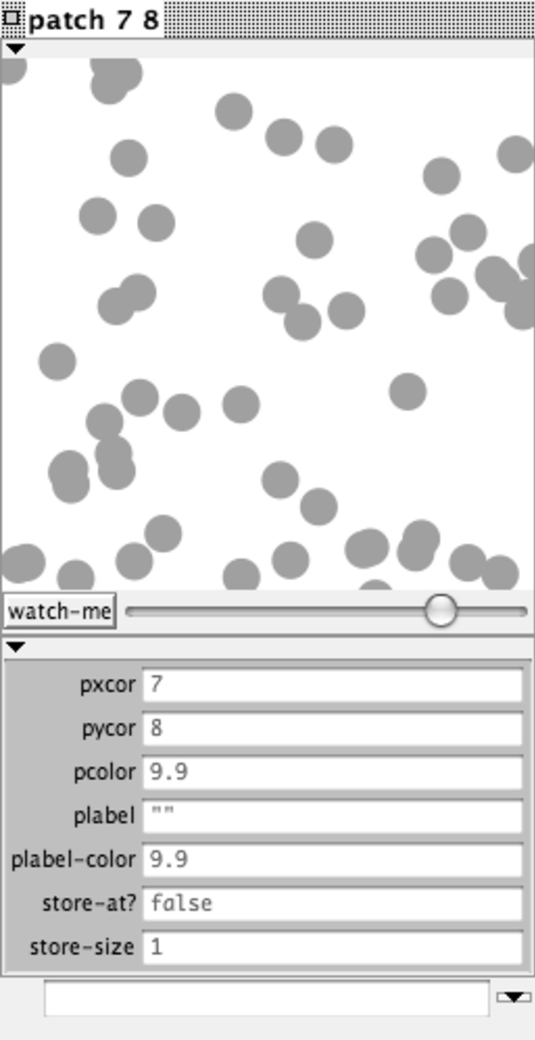
\includegraphics[width=3in]{figures/HuffInspectPatch_7_8.pdf}  
   \caption{Inspecting the patch at position [7 8] of the Huff NetLogo model.} % using random-seed 22478
   \label{fig:Huff:inspecting_patch_7_8}
\end{figure}



\begin{figure}[htbp] %  figure placement: here, top, bottom, or page
   \centering
   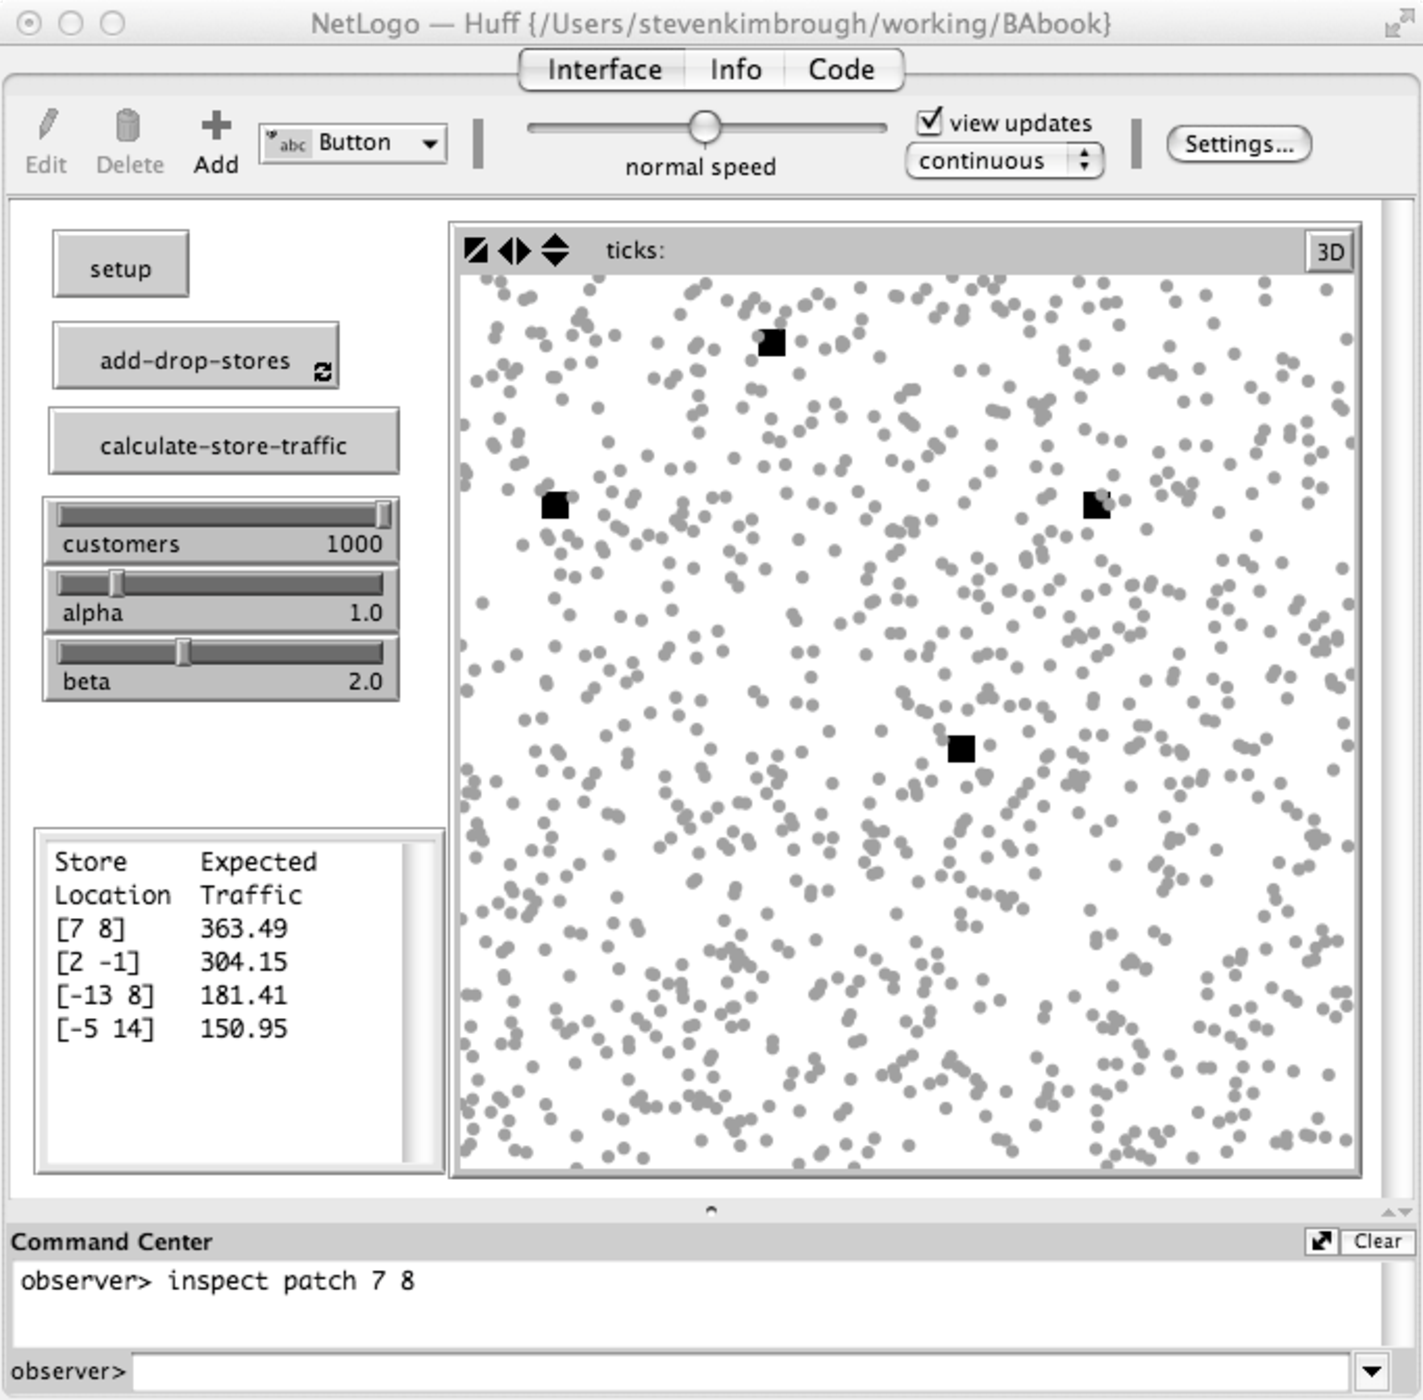
\includegraphics[width=\textwidth]{figures/Huff_increased_store_size.pdf}  
   \caption{Huff NetLogo model with size 2 for the store at 7 8, and otherwise the original values.} % using random-seed 22478
   \label{fig:Huff_increased_store_size}
\end{figure}

\newpage\clearpage

\subsection{Design \&\ Encoding 2}

% using random-seed 22478

The Huff Turtle-Based NetLogo model, Figure \ref{fig:HuffTurtleStart}, reimplements the Huff NetLogo model with one crucial design difference: stores are now represented as NetLogo turtles rather than as NetLogo patches. (Trivially, but usefully, stores are presented as buidling-suggestive icons, rather than as solid squares.) Notice that the basic setup and results exactly duplicate Figure \ref{fig:huffnlogo} for the original Huff NetLogo model.   Having stores be turtles makes it much easier to program them to move about, for patch agents in NetLogo cannot move. This presents us with opportunities to add useful features to the NetLogo model. Figure \ref{fig:HuffTurtleStart}, in consequence, has the look of a genuine analytics dashboard. We shall explore the new features in the next section. 


\begin{figure}[htbp] %  figure placement: here, top, bottom, or page
   \centering
   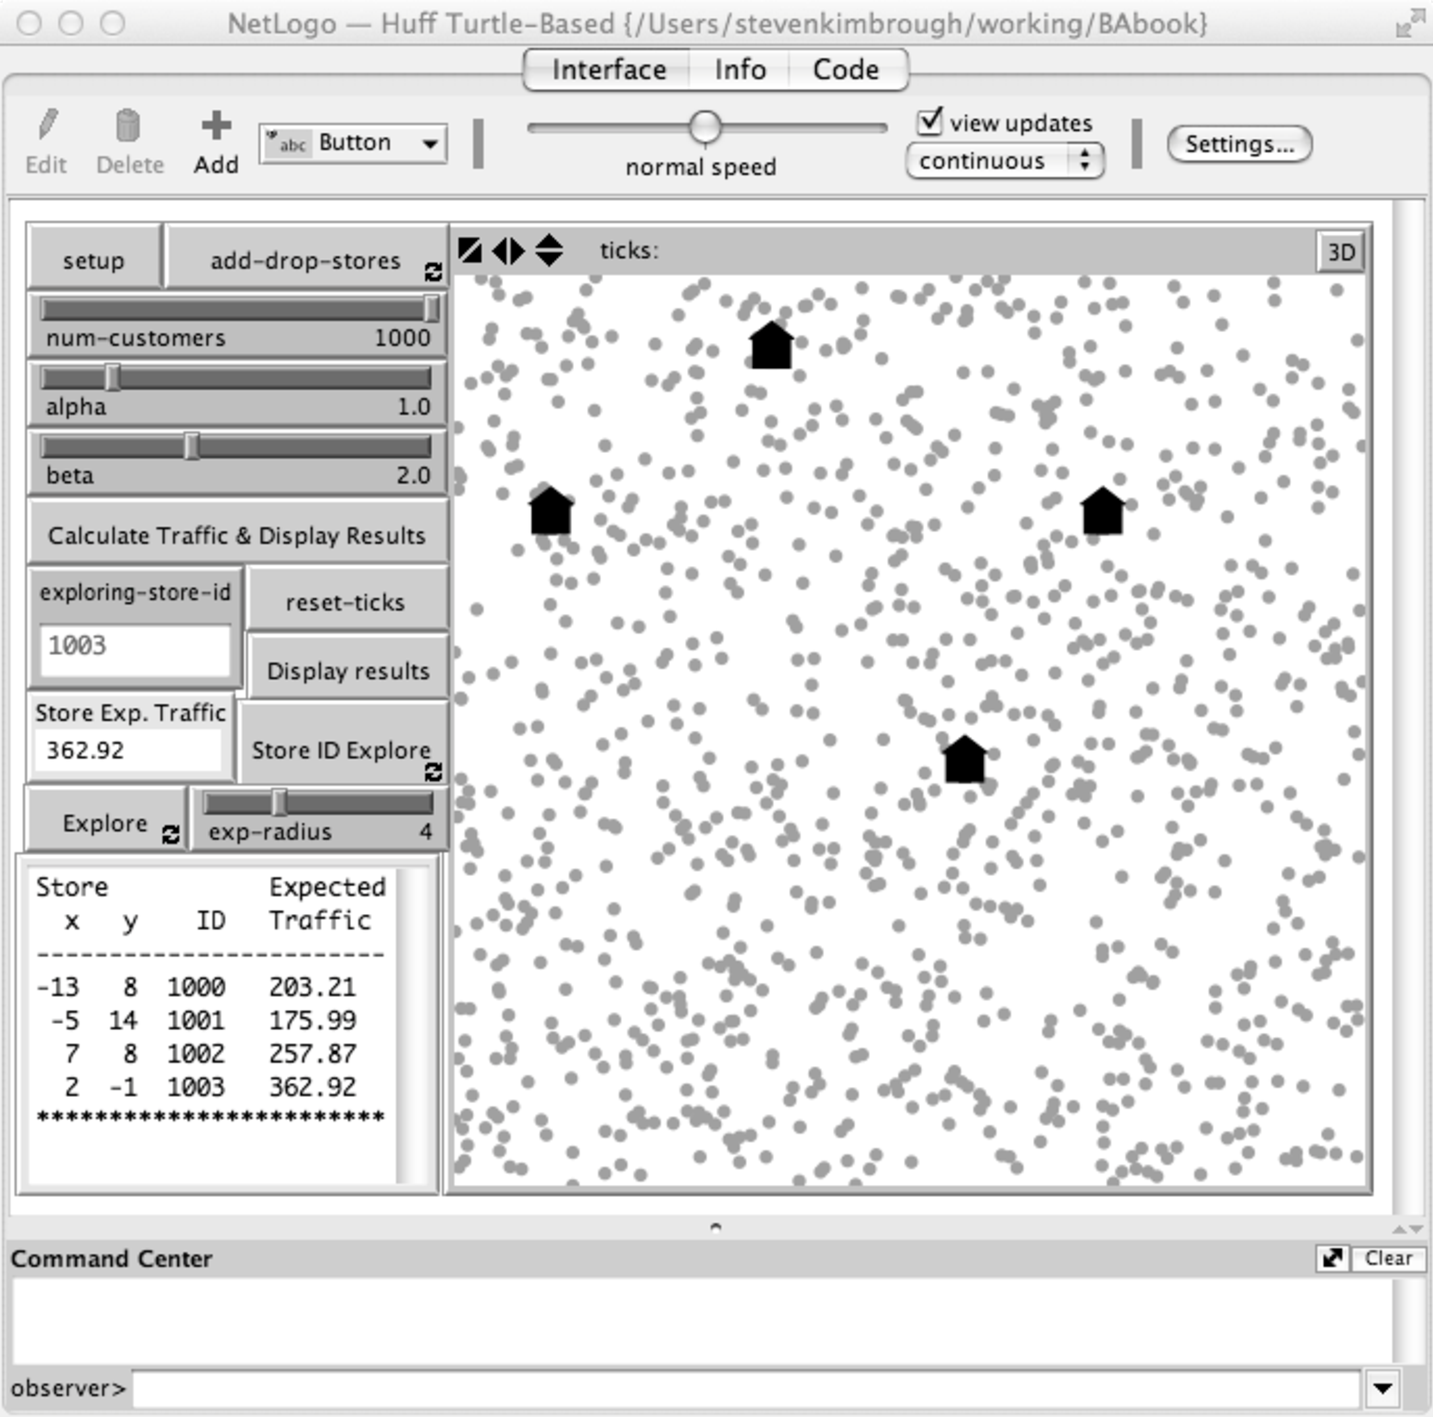
\includegraphics[width=\textwidth]{figures/HuffTurtleStart.pdf}  
   \caption{Huff Turtle-Based model, a NetLogo implementation of Huff's model. The basic setup and results exactly duplicate those of the Huff model in Figure \ref{fig:huffnlogo}} % using random-seed 22478
   \label{fig:HuffTurtleStart}
\end{figure}

\newpage
\subsection{Employment 2}

The program file for the Huff Turtle-Based NetLogo model is {\it Huff Turtle-Based.nlogo.}\index{Huff-Turtle-Based.nlogo@{\it Huff-Turtle-Based.nlogo}} It is available at the book's web site and at the NetLogo Modeling Commons 
 \url{http://www.modelingcommons.org}.\index{Modeling Commons}
 To run the program you will need to download and install NetLogo on your computer.
The NetLogo home page is \url{https://ccl.northwestern.edu/netlogo/}.\index{Netlogo!home page} There, you can download NetLogo and access a rich corpus of information about NetLogo.

Let us reconsider in our new environment  the post-solution analysis and deliberation case we explored for the original Huff NetLogo model (in \S\ref{sec:Huff:employment_1}): three incumbent stores share the current environment, a new store is known to be coming in, what are the consequences and what might be done?  

\begin{enumerate}
\item Edit the input widget exploring-store-id so that it contains 1002.
\item Click the reset-ticks button.
\item Adjust the exp-radius slider to have a value of 3.
\item Click the Store ID Explore button.
\item Watch while the store moves around and the tick counter increases. 
\item Click the Store ID Explore button to halt search when {\tt ticks} reaches, say, 40.
\item Click the Display results button.
\end{enumerate}
When you are done the results should look something like Figure \ref{fig:HuffTurtle1002Explore} (Of course your results will differ because you are using a different stream of random numbers.) Notice that store has improved its traffic position significantly, to 315, much better than the 276 we found in Figure \ref{fig:HuffMove1pdf}.  How did store 1002 do it? Time proceeds by ticks (or a notional clock). At each tick, the store randomly picked a spot within a radius of three patches (the value of {\tt exp-radius}) from its current position. It then had the global store traffic calculations redone. If the store 1002's expected traffic increased with the move, it retained the move; otherwise, it moved back to where it was at the start of the tick and restored the original traffic values. This completes the tick. The process was repeated until we stopped it at 41 ticks.  For future reference, this procedure is an example of \emph{greedy hill climbing}.\index{greedy hill climbing}\index{metaheuristics!greedy hill climbing} See Chapter \ref{COM_intro} for more information on greedy hill climbing. In the interim we hope it is obvious to you that this search procedure is aptly named.




\begin{figure}[htbp] %  figure placement: here, top, bottom, or page
   \centering
   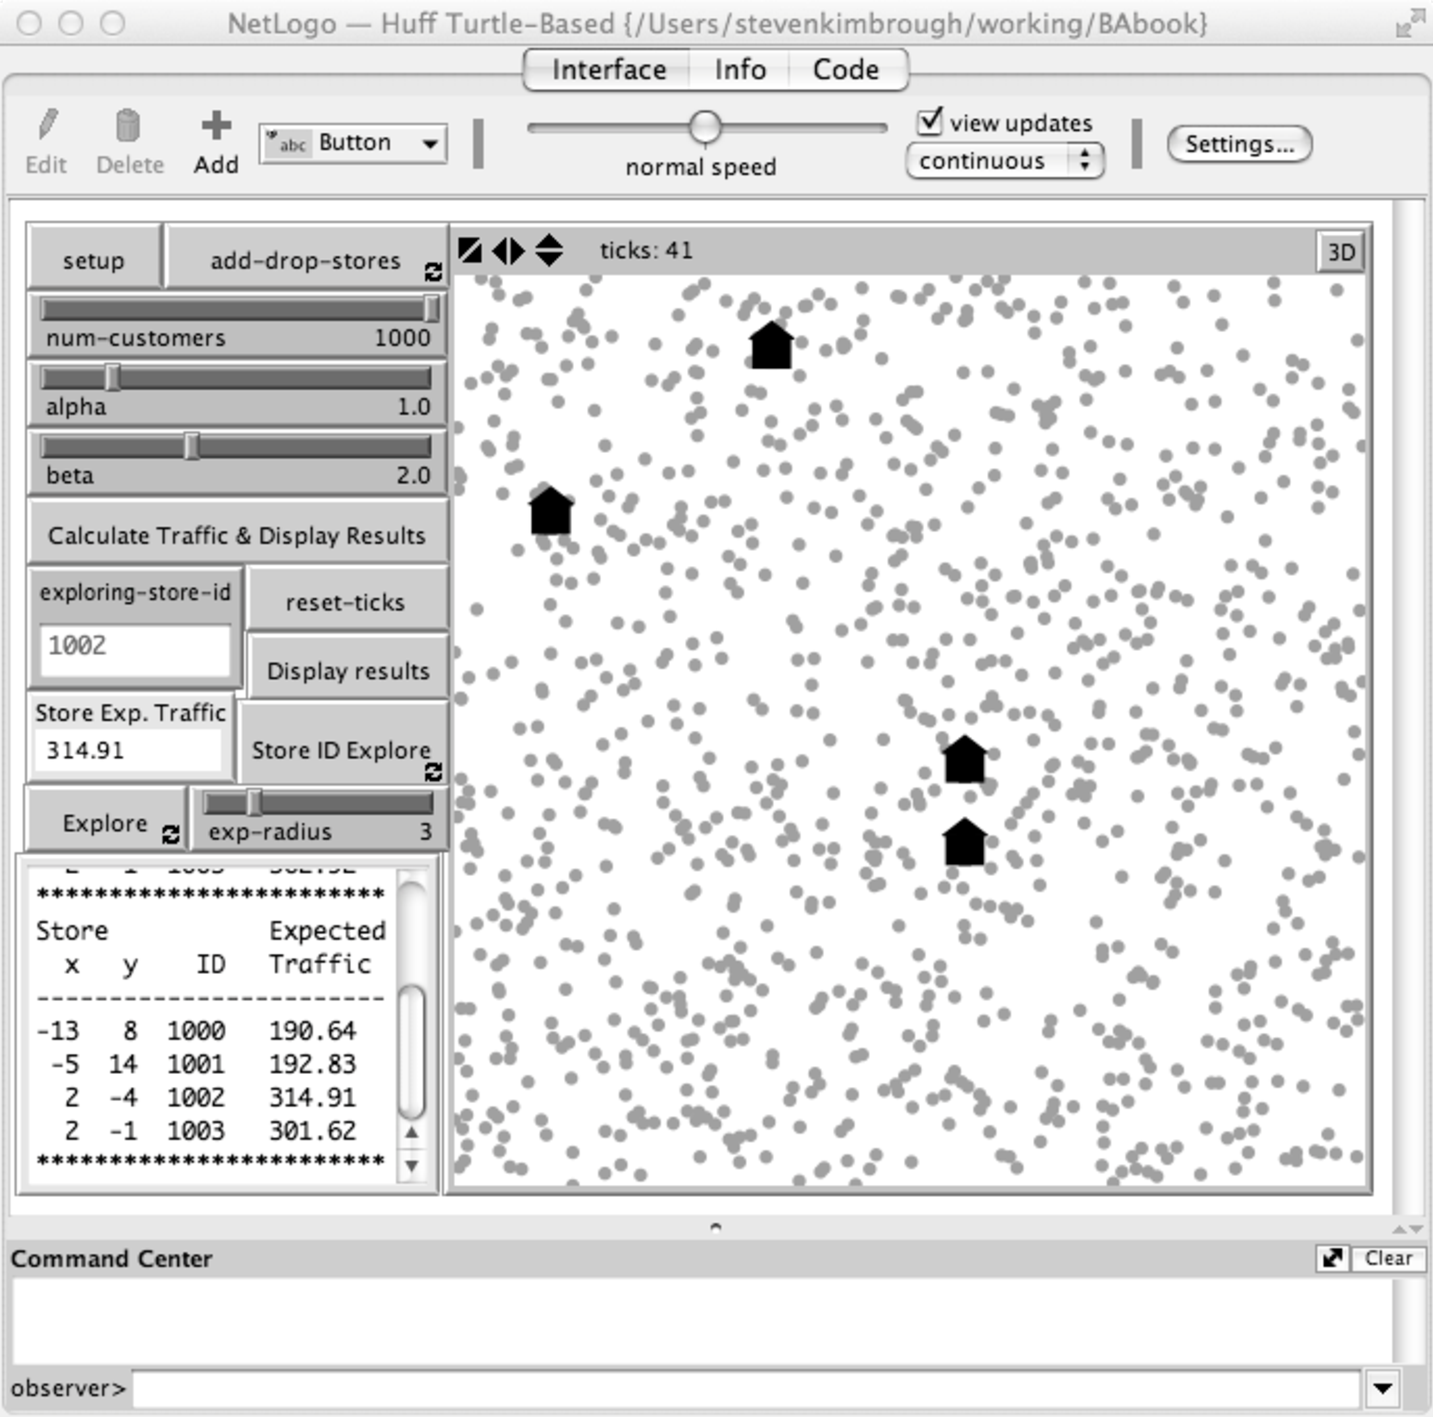
\includegraphics[width=\textwidth]{figures/HuffTurtle1002Explore.pdf}  
   \caption{Huff Turtle-Based model, configuration descended from that of Figure \ref{fig:HuffTurtleStart} after exploration by store 1002.} % using random-seed 22478
   \label{fig:HuffTurtle1002Explore}
\end{figure}

\newpage\clearpage

Now let's see what happens if all of the stores engage simultaneously in searching for better deals for themselves. 
\begin{enumerate}
\item Type {\tt ask store 1002 [setxy 7 8]} at the {\tt observer>} prompt and press Enter/Return on your keyboard. This restores 1002 to its original position.
\item Click the Calculate Traffic \&\ Display Results. This restores the output widget to its original message.
\item Click the reset-ticks button. This starts our clock anew.
\item Retain the exp-radius slider at the value of 3.
\item Click the Explore button.
\item Watch the stores move as the ticks counter increases.
\item Click the Explore button again after movement has halted. We did this when {\tt ticks} equaled 27 (resulting in it stopping at 28).
\item Click the Display results button.
\end{enumerate}
Your results should look something like Figure \ref{fig:HuffTurtleAllExplore}.



\begin{figure}[htbp] %  figure placement: here, top, bottom, or page
   \centering
   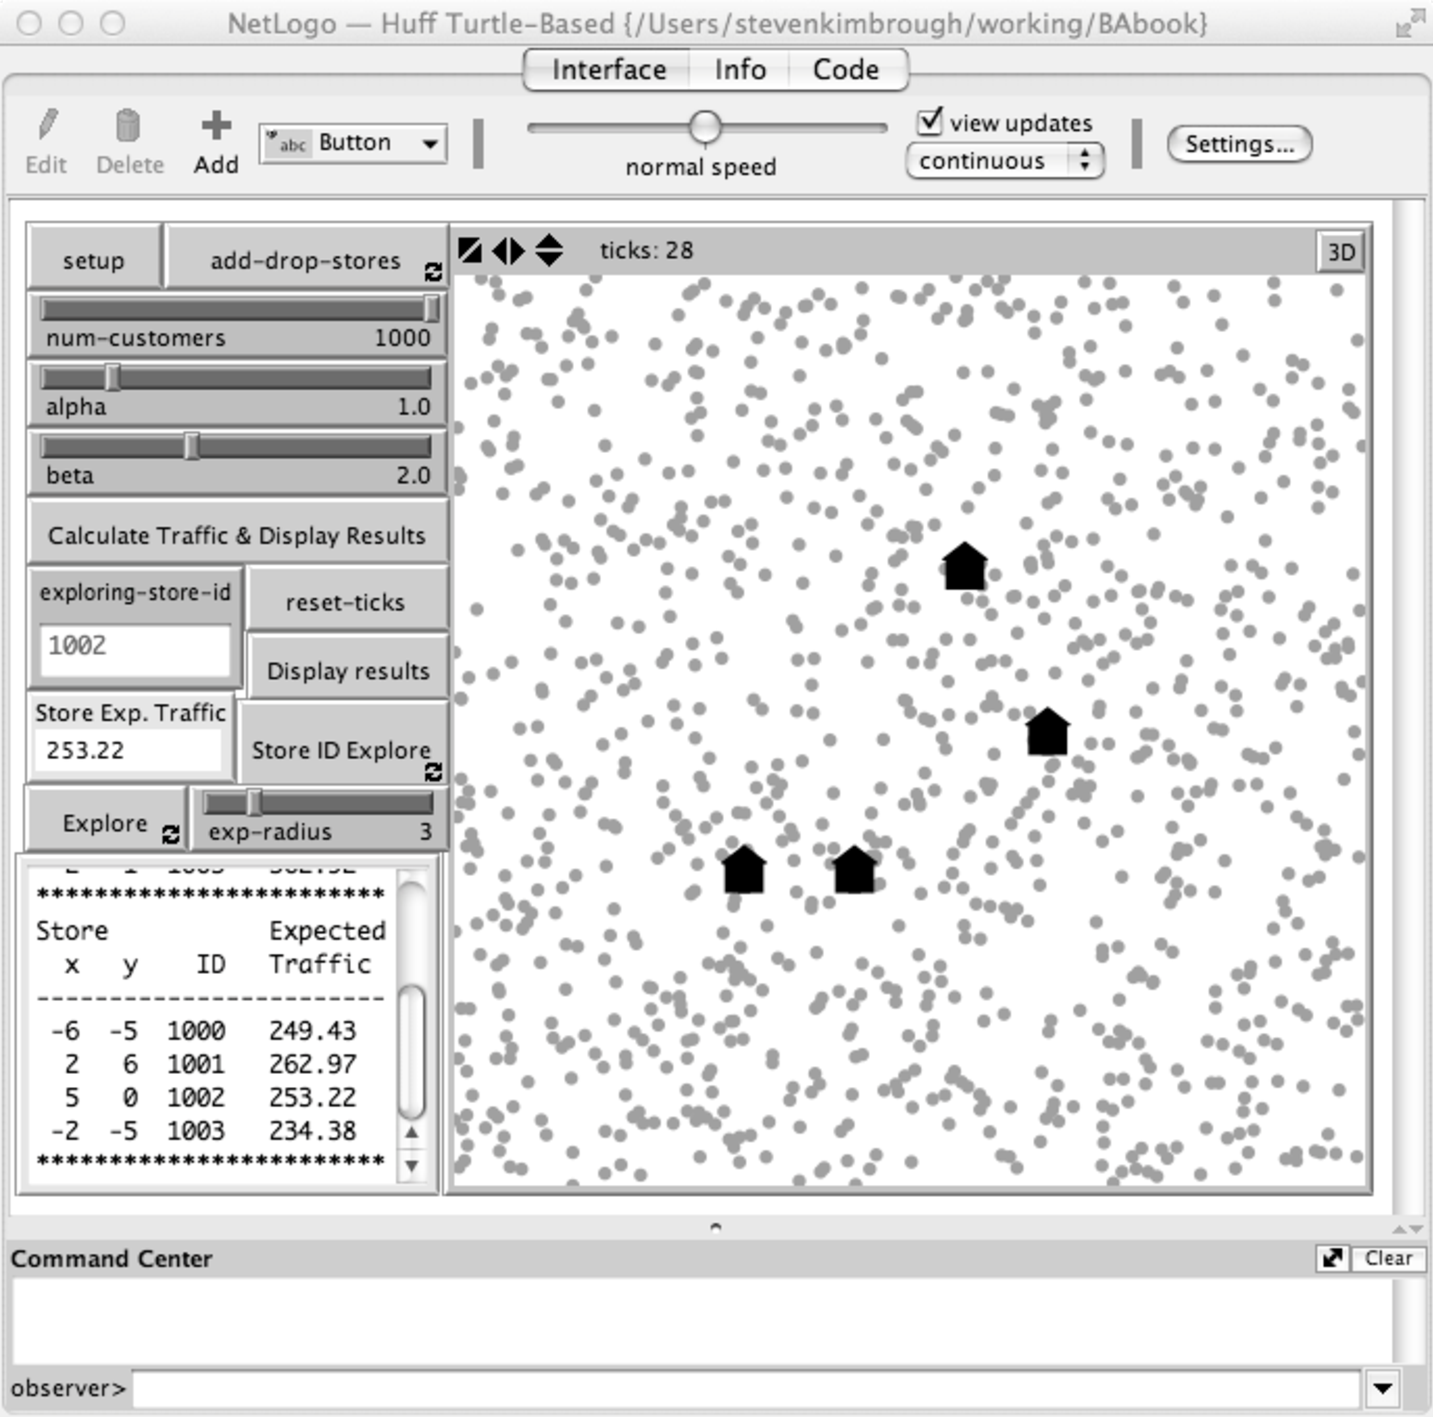
\includegraphics[width=\textwidth]{figures/HuffTurtleAllExplore.pdf}  
   \caption{Huff Turtle-Based model, configuration descended from that of Figure \ref{fig:HuffTurtleStart} after exploration by all stores simultaneously.} % using random-seed 22478
   \label{fig:HuffTurtleAllExplore}
\end{figure}
\newpage\clearpage


Finally, we repeated the last experiment after doubling the size of store 1001 to 2, keeping the other stores at size 1. Figure \ref{fig:HuffTurtleAllExplore1001Size2} shows the results.



\begin{figure}[htbp] %  figure placement: here, top, bottom, or page
   \centering
   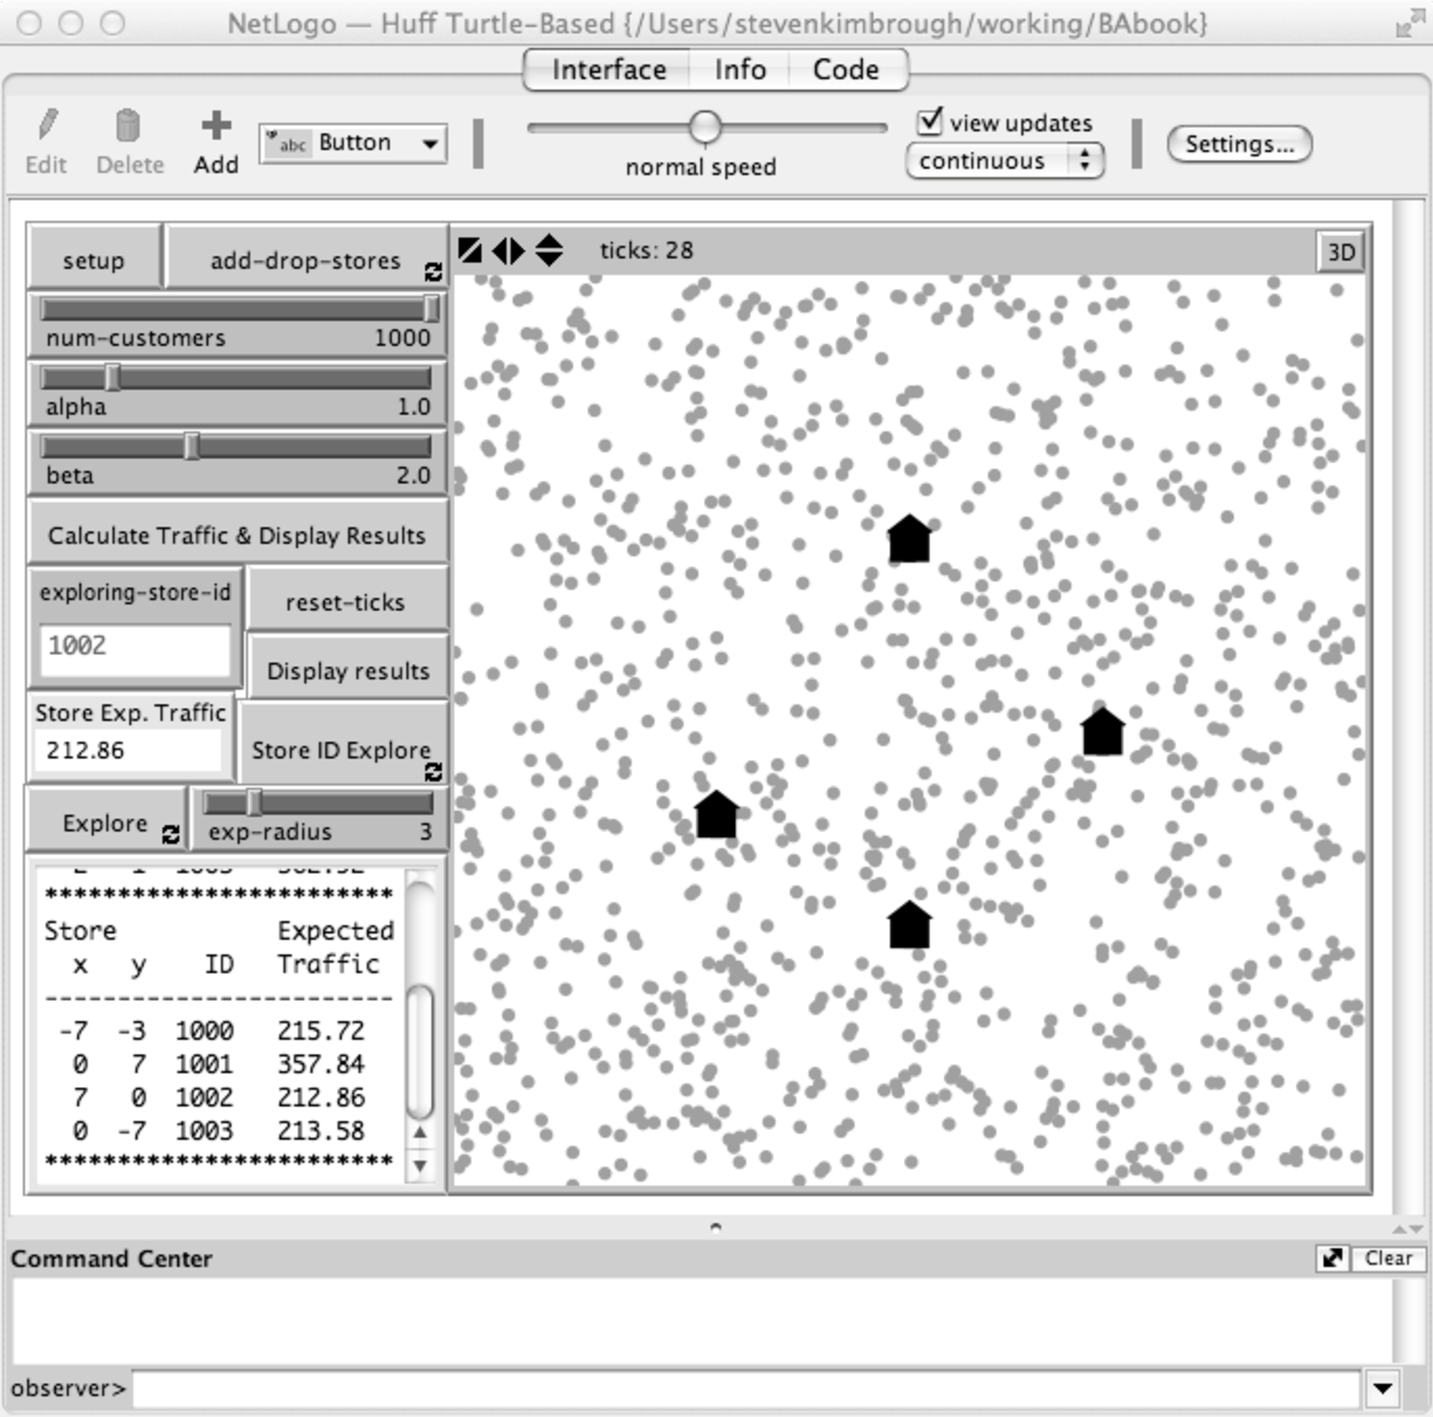
\includegraphics[width=\textwidth]{figures/HuffTurtleAllExplore1001Size2.pdf}  
   \caption{Huff Turtle-Based model, configuration descended from that of Figure \ref{fig:HuffTurtleStart} after exploration by all stores simultaneously but with store 1001 having a size of 2 (with 1 for the others).} % using random-seed 22478
   \label{fig:HuffTurtleAllExplore1001Size2}
\end{figure}
\newpage\clearpage


\section{Discussion\label{sec:huff_discussion}}

Decision making contexts can be divided cleanly into two kinds. In \emph{parametric} decision making\index{parametric decision} the decision maker has a number of choices, picks one of them, and receives a reward (positive or not) depending upon how Nature disposes.  Nature may be capricious, may behave randomly, but Nature is indifferent to the decision maker. Nature does not have her own interests nor does she care about the interests of anyone else. In \emph{strategic} decision making\index{strategic decision} there are always at least two decision makers. Any one decision maker has a number of choices, picks one of them, and receives a reward (positive or not) depending upon how Nature disposes \emph{and} on how any other decision makers choose. So, strategic decision making is also aptly known as \emph{interdependent decision making}\index{interdependent decision} because the decision makers are dependent upon each other, in part, for what happens.

Converse's formula, or at least our use of it, is straightforwardly for parametric decision making. There is city $A$ with its existing store, what will be our traffic if we install a store in city $B$? The answer for the question as formulated depends only on Nature. With our treatment of the Huff model, especially in the Huff Turtle-Based NetLogo implementation, we are well within the territory of strategic decision making.

With these brief preparatory remarks to hand we continue the discussion in the next section.



\section{For Exploration}

\begin{enumerate}
\item Under what sorts of conditions is it likely that an organization facing a store location problem can do its market area analysis largely without regard to strategic considerations (that is, without having to take into account possible decisions by competing firms)?
\item Under what sorts of conditions is it likely that an organization facing a store location problem can do its market area analysis largely without neglecting strategic considerations (that is, without being able to ignore possible decisions by competing firms)?
\item Use the Huff NetLogo model to find the best position you can for the store that is originally located at [7 8]. That is, repeat the experiment we reported in Figure \ref{fig:HuffMove1pdf}. What do you find?
\item Consider the generally good positions that you see for the store in the experiment we reported in Figure \ref{fig:HuffMove1pdf}. Characterize them. Do you see any patterns?
\item What justification can you give for the positive role of store size in the Huff model? 
\item Characterize and explain the result of the experiment resulting in Figure \ref{fig:HuffTurtle1002Explore}.
\item Characterize and explain the result of the experiment resulting in Figure \ref{fig:HuffTurtleAllExplore}. 
\item Characterize and explain the result of the experiment resulting in Figure \ref{fig:HuffTurtleAllExplore1001Size2}. 

\item Characterize and compare the results of the experiments behind Figures \ref{fig:HuffTurtleAllExplore} and \ref{fig:HuffTurtleAllExplore1001Size2}. 

\item Read up on the Hotelling model(s) for store location. See in particular the {\it Hotelling's Law.nlogo} model, which is in the Models Library that ships with NetLogo.  Compare and contrast what we learn from it versus the Huff model implemented as {\it Huff Turtle-Based.nlogo.}

\item Design new experiments to conduct with the Huff Turtle-Based model to explore the effect of store size on the outcome of exploratory search by all stores.
\item Design new experiments to conduct with the Huff Turtle-Based model. Look at more or fewer  stores, different values of $\alpha$ and $\beta$, non-random distributions of customers, and so on.
\item Discuss how you might go about conducting a real world study using the Huff Turtle-Based model.  How would you map real customer locations to the model? What sorts of problems might you expect to have in building such a model?  Under what conditions do you think the resulting model, admittedly imprecise in its representation, would be useful?
\end{enumerate}

\section{For More Information}

% The book's web site is\newline

% \noindent\website .\newline

\noindent There, in the {\it NetLogo/} directory you will find the NetLogo programs we mention in conjunction with the chapter: {\it Converse Formula.nlogo} and {\it Huff Interactive.nlogo.} These files are also available online at \url{http://www.modelingcommons.org}.\index{Modeling Commons}

The NetLogo home page is \url{https://ccl.northwestern.edu/netlogo/}.\index{Netlogo!home page} There, you can download NetLogo and access a rich corpus of information about NetLogo.

On market area analysis, and the Huff gravity model:
\begin{enumerate}
\item {\tt http://www.directionsmag.com/articles/}-\newline
{\tt retail-trade-area-analysis-using-the-huff-model/123411}
\item Huff, D.L., 2003. Parameter Estimation in the Huff Model. ArcUser, October-December, 34--36.
\url{http://www.esri.com/news/arcuser/1003/files/huff.pdf}
\item Two videos about using the GIS Maptitude to do Huff models.

\url{http://www.youtube.com/watch?v=9d0Ccsj2Ct4}

\url{http://www.youtube.com/watch?v=pOfz4d2un28}
\end{enumerate}

%YouTube video from Eric Huff, interesting but not related to the Huff model: 
%\url{http://www.youtube.com/watch?v=Ll0NIidKiIg}
%
%Mod-05 Lec-10 Models of Consumers and Models of Consumer Behaviour,
%\url{http://www.youtube.com/watch?v=6MqMt5D0JLg}

{\it Foundations of Location Analysis,}  edited by Eiselt and Marianov, has an excellent historical chapter pertaining to the Huff model as well as Converse's formula \cite[Chapter 18]{eiselt_marianov_eds_2011}.

The literature on agent-based modeling is burgeoning. Still very much worthwhile and highly recommended is {\it Growing Artificial Societies} by Epstein and Axtell \cite{epstein_axtell_1996}.
{\it Agent-Based and Individual-Based Modeling} by Railsback and Grimm \cite{railsback_gramm_netlogo_2012} provides excellent tutorial material and is based in NetLogo.

\ifnum\draft=1
\vfill
\noindent File: Huff.tex
\fi
